\chapter{Revisão da literatura}

\cite{echer2001revisao} argumenta sobre a imprescindibilidade da revisão da literatura para a elaboração do trabalho científico, pois é preciso ter ideia clara do problema a ser resolvido. Como consequência, agrupar-se-ão neste capítulo as análises similires ao achados nos demais capítulos.

\subsubsection{Correlação do EGDI com o PIB}

\cite{alisherovna2021whether} chegou a uma conclusão similar na figura \ref{fig:usmanova_egdi_gdp} a da figura \ref{fig:dispensao_egov_pib}, porém o autor adotou a taxa de crescimento do PIB ao invés do PIB \textit{per capita} PPC.

\begin{figure}[H]
	\centering
	\caption{Como os países se posicionam em relação ao EGDI de acordo com sua taxa de crescimento do PIB}
	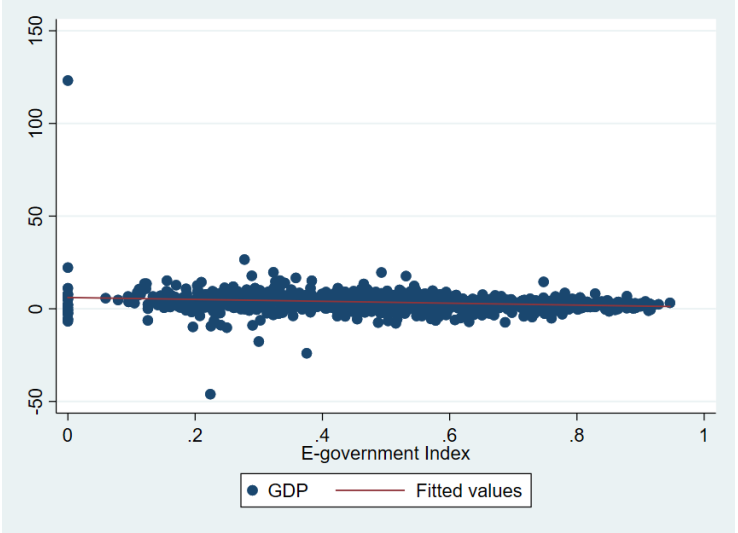
\includegraphics[width=1\linewidth]{figuras/egdi/usmanova_egdi_gdp}
	\label{fig:usmanova_egdi_gdp}
	\footnotesize{Fonte: \cite{alisherovna2021whether}}
\end{figure}

Embora a figura \ref{fig:usmanova_egdi_gdp} mostre menos pontos extremos do que a figura \ref{fig:dispensao_egov_pib}, percebe com o PIB, seja \textit{per capita} PPC ou sua taxa de crescimento tem forte correlação com o EGDI. 

Complementarmente, \cite{kumar2020cultural} descobriu que o desenvolvimento econômico, mensurado pelo PIB \textit{per capita}, significativamente e positivamente impulsiona o EGDI. 

\subsubsection{EGDI e governo eletrônico}

\cite{kotenok2020government} conclui que o impacto do governo eletrônico pode impulsionar a inovação ou até mesmo ser um componente importante para entender como a economia é transformada devido à tecnologia. 

\subsubsection{Governo eletrônico}

\cite{ziolo2022government} cita que na União Europeia (até 2020), observou-se a correlação observada entre o nível de desenvolvimento do governo eletrônico e as áreas ambiental, social e econômica parece ser de grande importância. Essa correlação implica que a digitalização dos processos administrativos pode ter um impacto real no desenvolvimento sustentável, promovendo, assim, mudanças positivas em todas as suas três esferas.
